%-----------------------------------------------
% Template para criação de resumos de projectos/dissertação
% jlopes AT fe.up.pt,   Fri Jul  3 11:08:59 2009
%-----------------------------------------------

\documentclass[9pt,a4paper]{extarticle}

%% English version: comment first, uncomment second
%\usepackage[portuguese]{babel}  % Portuguese
\usepackage[english]{babel}     % English
\usepackage{graphicx}           % images .png or .pdf w/ pdflatex OR .eps w/ latex
\usepackage{times}              % use Times type-1 fonts
\usepackage[utf8]{inputenc}     % 8 bits using UTF-8
\usepackage{url}                % URLs
\usepackage{multicol}           % twocolumn, etc
\usepackage{float}              % improve figures & tables floating
\usepackage[tableposition=top]{caption} % captions
%% English version: comment first (maybe)
\usepackage{indentfirst}        % portuguese standard for paragraphs
%\usepackage{parskip}

%% page layout
\usepackage[a4paper,margin=30mm,noheadfoot]{geometry}

%% space between columns
\columnsep 12mm

%% headers & footers
\pagestyle{empty}

%% figure & table caption
\captionsetup{figurename=Fig.,tablename=Tab.,labelsep=endash,font=bf,skip=.5\baselineskip}

%% heading
\makeatletter
\renewcommand*{\@seccntformat}[1]{%
  \csname the#1\endcsname.\quad
}
\makeatother

%% avoid widows and orphans
\clubpenalty=300
\widowpenalty=300

\begin{document}

\title{\vspace*{-8mm}\textbf{\textsc{Journata - Designing the interaction of a mobile application for exchanging public transport information among travellers}}}
\author{\emph{Marco André Moreira Amador}\\[2mm]
\small{Project/Dissertation performed under guidance from \emph{Prof.\ Teresa Galvão Dias}}\\
%\small{na \emph{FazSoft Lda}}
}
\date{23th June 2014}
\maketitle
%no page number 
\thispagestyle{empty}

\vspace*{-4mm}\noindent\rule{\textwidth}{0.4pt}\vspace*{4mm}

\begin{multicols}{2}

\section{Motivation}\label{sec:motiva}

Nowadays, the utilization of mobile devices with Internet access allow users to use several kinds of applications anytime and at any given moment, and to read and share various types of information in real time.

Following that, it was previously proposed the creation of a mobile application for sharing public transport information in real time. 

This application is very innovative, since the shared information has origin in the users of the platform, who submit information to be seen by other users, about the trip or vehicle driver.

Other innovation consists in the way users are connected between themselves, through the creation of dynamic social networks (in time and space), centred in the user.

This work aims to improve the interface and interaction of the previously developed application, making it more attractive, in order to improve the experience of utilization of public transportation networks by travellers, and trying to eliminate the waiting times or make them more bearable.

\section{Goals}\label{sec:goals}

Following the aspects mentioned in the previous section, this work aims to develop an user interface for the mentioned application, while achieving the following objectives:

\begin{itemize}
\item Create and analyse appropriate metaphors for the interaction with dynamic social networks.
\item Design and test innovative visual affordances for the concept of dynamic social networks.
\item Apply state-of-the-art concepts related with Human-Computer Interaction in order to maximize the usability of the application by its final users, while addressing usability problems identified on the previous existing prototype.
\item Develop a functional prototype for an Android mobile application based on the obtained solutions.
\item Test the system and evaluate the results obtained. 
\end{itemize}

\section{Problem Description and Approach}\label{sec:work}

Having in consideration that the information in the platform is shared between users, the usability of the application is crucial to its success and adoption between public transport users.

In that sense, it is important to choose a development process that includes final users and usability experts in validation and evolution of the performed work.

The choice fell upon the following four-phased process:
\begin{itemize}
\item \textbf{\emph{Definition of Usability Requirements}} - Includes analysis of usability limitations encountered in a previous iteration of the application, the creation of design solutions in order to solve those limitations, and the discussion of said solutions in a focus group session performed among potential users of the application.

\item \textbf{\emph{Design}} - Creation and iterative evolution of alternative designs for the application interface, recurring to low-level prototypes.

\item \textbf{\emph{Prototyping}} - Development of a functional prototype in \emph{Android} following the work performed in the previous phase.

\item \textbf{\emph{Evaluation}} - Realization of usability evaluation and testing, and analysis of the obtained results.
\end{itemize}


\subsection{Requirements Elicitation}\label{sec:req}

The mentioned application had a previously well defined set of features, including:

\textbf{-} Check-in and checkout in a vehicle/trip;

\textbf{-} Viewing a news feed with information from the vehicle/route;

\textbf{-} Comment submission;

\textbf{-} Rating of other users' comments;

\textbf{-} Planning a journey for a near future.

After an initial analysis, it was concluded that the check-in and check-out in a vehicle/route features possibly had low visibility to the user, giving the high time for the execution of those tasks that was registered in previously performed tests. At the same time, similar results related to the rating comments feature pointed to a difficulty from users in grasping the concept and the need to have and use that feature.

Initial design solutions for several navigation components and features of the application were then conceived, aiming to reduce those limitations. Those solutions were meant to be presented in a focus group session with potential users, aiming to define additional usability requirements for the application and understand the users' needs.

The session revealed two big limitations in the conception of the application, conditioning the information obtention needs manifested by the users: the impossibility of receiving information from a vehicle/route before checking-in in that vehicle/route, in order to perform an informed travel decision beforehand and consider alternative transport options, and the impossibility to receive information from more than one route/vehicle simultaneously.

\section{Application Development}

In this phase, the attribution of a name - \textbf{Journata} - and a logo to the application were discussed. Several alternative designs for the several components and modules of the application were also conceived (and improved through an iterative process), through the appliance of usability guidelines for mobile devices.

Apart from improvements in the usability and interaction that were introduced, several new features were created following needs revealed by users, also facilitating their understanding of the application. Some deep changes regarding the implementation of the concepts behind the application were also performed, such as:

\begin{itemize}
\item It is now possible to receive information from several routes simultaneously, through the subscription of feeds that do not require user check-in.

\item Changes to the representation of the concept of 'network' in the interface of the application, making it closer to the concept proposed in theory. Subscribing a feed between a point A and another point B now displays information about all the transportation options between A and B to the user.

\item Creation of lists of favourite and scheduled journeys.

\end{itemize}

In order to validate the conceived interface before an implementation phase, an usability test was performed among some users, that accomplished a very well defined set of tasks. This test alerted to the need of simplifying the system of rating other users' comments, leading to another introduced change - a new point system to quantify the reliability of the users' comments.

The implementation phase followed the designs conceived in the previous phase, as it is possible to see in Fig. 1.

\begin{figure}[H]
\centerline{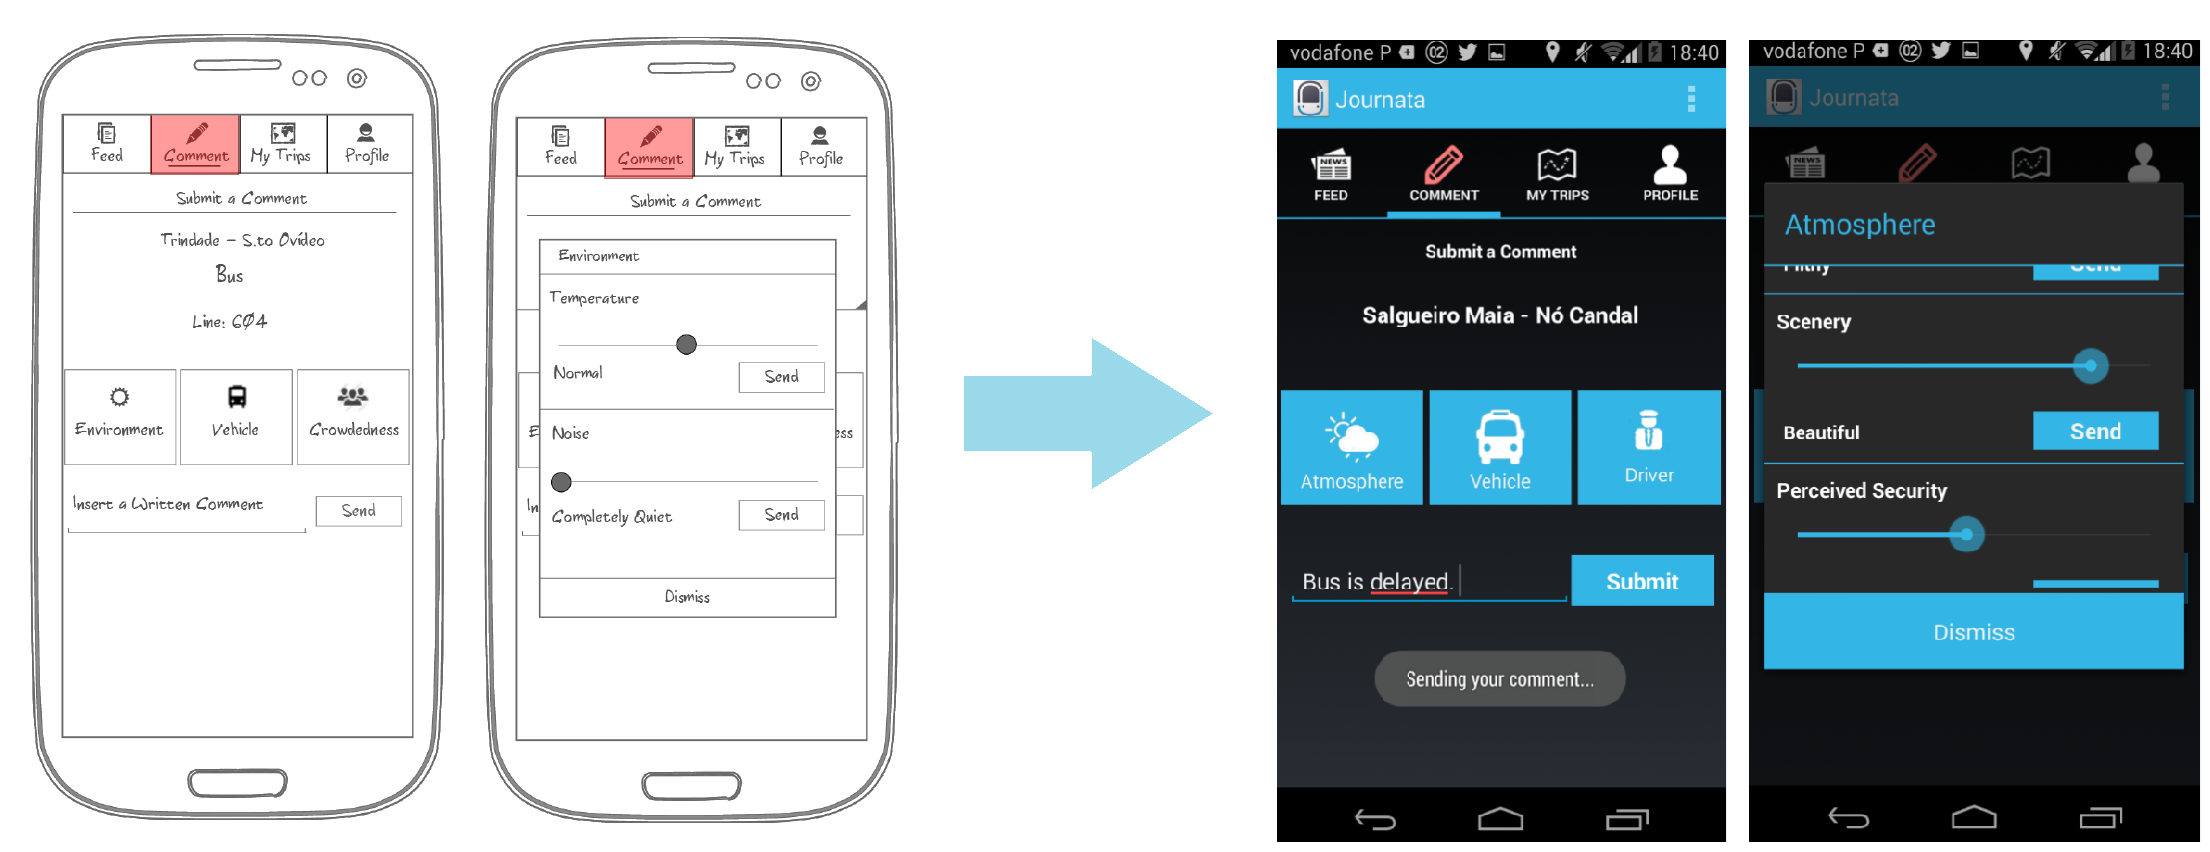
\includegraphics[scale=.15]{artigo.png}}
\caption{Design e implementation of the comment submission feature.}  
\label{fig:figura}
\end{figure}


\section{Tests and Results}

After the implementation phase, a test session among experts in the fields of usability and mobile application development for public transports was performed. Those experts validated the process used to perform this work, recognizing the easy use of the application.

As a result of the session, several contributions and recommendations regarding the interaction inside the application were given, and should be followed and implemented in a future iteration.

The session also allowed the discussion of several aspects of the application, such as the new feedback point system, or the possibility of aggregation several comments in one, that should be explored with depth in the future and discussed among potential users.

\section{Conclusions}\label{sec:conclui}

After the realization of this work, it is concluded that the new iteration of the application consists in a big step towards the right direction, confirming the great potential of the project. There are, however, several aspects to be explored in the future.

\subsection{Future Work}

The development of the application will continue in the scope of a project for the development of a large-scale solution involving mobile payments in public transports, aiming to dematerialize transport tickets.

The necessity of improving the data architecture supporting the application is recognized, in order to allow the proper working of some of the changes introduced in this work. 
The introduced of data-mining techniques to deduce users' travel patterns would also bring added value to the application.

Finally, it is discussed the integration of \textbf{Journata} with some existing social networks, and with other applications related to public transportation, in a perspective that aims to eliminate the check-in process by replacing it with a process of automatic validation inside vehicles (via \emph{NFC}, for instance).

%%English version: comment first, uncomment second
\bibliographystyle{unsrt-pt}  % numeric, unsorted refs
%\bibliographystyle{unsrt}  % numeric, unsorted refs
\bibliography{refs}

\end{multicols}

\end{document}
